\section{Methodology}
\label{sec:methodology}

To address the significant challenges of small object detection, particularly the loss of information from downsampling and the lack of surrounding context, we propose the Slicing-Aided Transformer Network (SAT-Net). Our method is not a single end-to-end model, but rather a novel inference pipeline that integrates three powerful techniques, as justified by our literature review: (1) Slicing-Aided Hyper Inference (SAHI) for preserving high-resolution detail, (2) a lightweight Super-Resolution (SR) network to restore spatial detail, and (3) a transformer-based detector with a bidirectional feature pyramid for robust feature extraction and fusion.

The complete pipeline is illustrated in Figure~\ref{fig:pipeline}. The subsequent sections describe each major component in detail.

\begin{figure}[H]
    \centering
    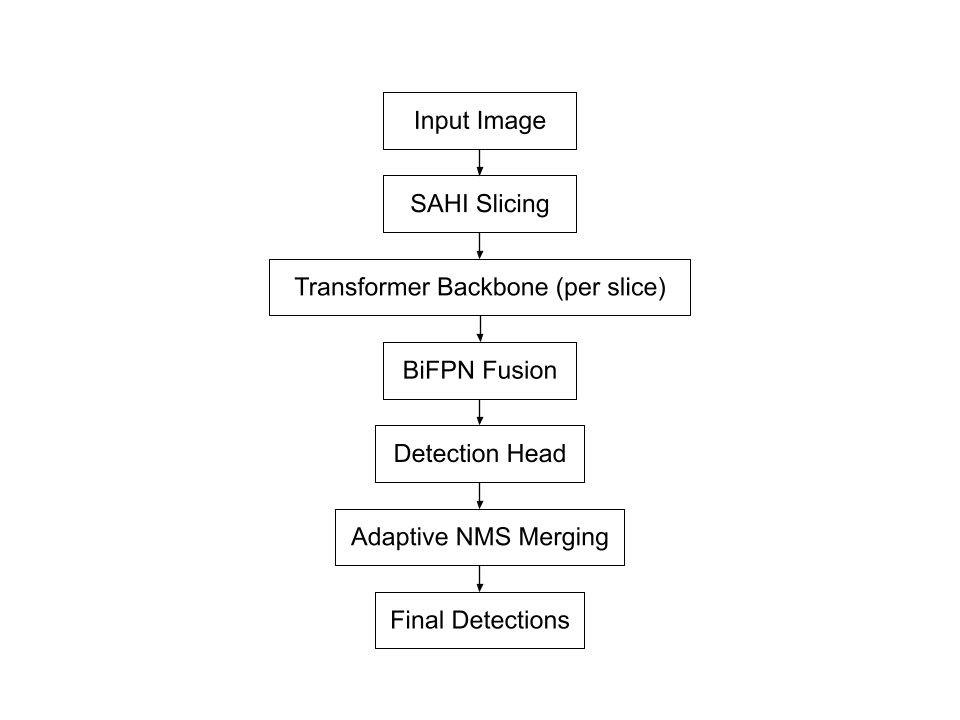
\includegraphics[width=0.9\columnwidth]{pipeline.png}
    \caption{The proposed SAT-Net inference pipeline.}
    \label{fig:pipeline}
\end{figure}

\subsection{High-Resolution Sliced Inference (SAHI)}

Traditional detectors must downsample large images (e.g., 2000$\times$1500 pixels) to fit memory constraints (e.g., 640$\times$640). For small objects (e.g., $32 \times 32$ pixels), this aggressive downsampling can erase them entirely.

To combat this, we adopt the core principle of Slicing-Aided Hyper Inference (SAHI)~\cite{aksoy2022slicing}. Instead of downsampling the entire image, we first slice the original high-resolution image into $N$ overlapping patches. We use a patch size of $640 \times 640$ pixels with a $25\%$ overlap. This ensures that inference is performed on high-resolution regions, allowing the detector to extract much richer features.

\subsection{Super-Resolution Enhancement}
\label{sec:sr_enhance}

While slicing preserves scale, the features of extremely small objects ($<20$ pixels) may still be too indistinct for a detector. As the second stage of our pipeline, we apply a lightweight super-resolution network (e.g., LightSRNet, inspired by \cite{li2025superresolution}) to each $640 \times 640$ patch before detection.

This step scales each patch by 2x to $1280 \times 1280$, recovering fine textures and sharpening edges. This enhancement provides the subsequent transformer backbone with higher-quality input, improving its ability to distinguish very small objects from background clutter.

\subsection{Transformer-based Detection and Fusion}

A detector processing one slice suffers from a lack of global context. To mitigate this, a highly robust feature extractor is required. We employ a transformer-based backbone, inspired by models like Deformable DETR~\cite{zhu2021deformable}. The self-attention mechanism is inherently designed to model long-range dependencies.

The features from the transformer are then fed into a Bidirectional Feature Pyramid Network (BiFPN)~\cite{tan2020efficientdet}. A BiFPN adds a bottom-up pathway to the standard top-down FPN, allowing low-level, high-resolution features to be repeatedly refined with high-level semantic context. This bidirectional flow is critical for small object detection.

\subsection{Pipeline Integration and Merging}

The complete SAT-Net methodology (Fig.~\ref{fig:pipeline}) integrates these components into a single inference pipeline:
\begin{enumerate}
    \item A high-resolution input image is received.
    \item The image is divided into $N$ overlapping $640 \times 640$ patches (SAHI).
    \item \textbf{Each patch is passed through the SR network, upscaling it to $1280 \times 1280$.}
    \item Each upscaled patch is passed independently through our detection model (Transformer backbone + BiFPN neck + anchor-free detection head).
    \item The bounding box coordinates from each patch's detections are mapped back to the original image's coordinate system.
    \item Due to the overlap, a final Adaptive Non-Maximum Suppression (NMS) is applied to the complete set of global detections to resolve duplicates.
\end{enumerate}